\section{Epilog}\label{sec:NFMEpilog}

\subsection{Erläuterung Epilog}
\paragraph{Nicht Teil dieser Strategie}
Im Epilog werden Themen behandelt, welche sich nicht in die Strategie einbinden lassen oder der Aufwand nicht aufgebracht werden kann oder möchte, nach einer Integration zu suchen. In der Weiterführung mit \gls{p_NFM} wird angenommen, dass mehr Themen behandelt werden, und hier einen Platz finden.\\

Sollte in der losen Ausführung erkannt werden, dass diese sinvoll unter \ref{sec:Erreichung} oder unter den Objectives integriert werden sollten oder diese ändern, wird der Abschnitt mit übernommen.

\paragraph{Concept Mapping}
Im weiteren Umgang mit dem \gls{p_NFM} Vorhaben, wird es viele weitere Gedanken dazu geben. Dieser Abschnitt soll dabei helfen, zwischen neuen Gedanken zu unterscheiden. Sind diese als leicht anderes Konzept zu verstehen oder als Erweiterung der bisherigen Logik oder sogar Revision der bestehenden. Bevor somit ganze Bereiche umgeschrieben werden, soll darüber nachgedacht werden, ob der neue Gedanke nur ein leicht anderes Konzept representiert, welches nur sprachlich gemappt werden soll, oder wirklich Änderungen an der bestehenden Arbeit vorgenommen werden muss.


\subsection{Recherche Entwicklungs Zeitverlauf}
\begin{enumerate}%[align=left,leftmargin=*,widest=10]
	\item[Geburt]
	\begin{itemize}
		\item Erster Atemzug: Zur Geburt wird durch einen Adrenalienschub die ungenutzten Lungen zur Atmung animiert.
		\item Muskeln Kontraktion: Muskeln müssen erste jetzt komplett die Funktion übernehmen.
		\item Herz: Dies hat zwei Löcher. Diese schließen sich in den ersten Tagen. Grund dafür ist, dass die Lungen jetzt mit Blut versorgt werden müssen, welches sie vorher nicht mussten.
		\item Erster Stuhlgang: Dieser besteht aus einer grünen Flüssigkeit, welcher sich aus der Verdauungsflüssigkeit ohne jegliche Nahrung besteht.
	\end{itemize}
	\item[1 Woche]
	\begin{itemize}
		\item Temperatur
		\begin{itemize}
			\item Körper von \gls{p_NFM} muss sich an eine neue Außentemperatur anpassen. Es kommt zu einem Temperaturabsturz von \SI{38}{\celsius} zu durchschnittlich \SI{18}{\celsius}.
			\item Der Hypothalamus ist bei neu geborenen nicht vollständig entwickelt, eine eigene Temperaturregulierung ist noch nicht möglich.
			\item Zusätzlich besitzen \gls{p_NFM} eine große Körperoberfläche im Verhältnis zum Körpervolumen. Dies verursachte einen hohen Temperaturverlust. 
			\item Gewinnung von Wärme aus Muskelkontratkion ist im ersten Jahr nicht möglich.
			\item Die Wärmentwicklung wird durch Braunefettzellen gesteuert. Diese Wärmequelle nimmt im ersten Lebensjahr ab, bis der Körper eigenständig die Wärmeregulierung übernehmen kann.
			\begin{figure}[H]
				\centering
				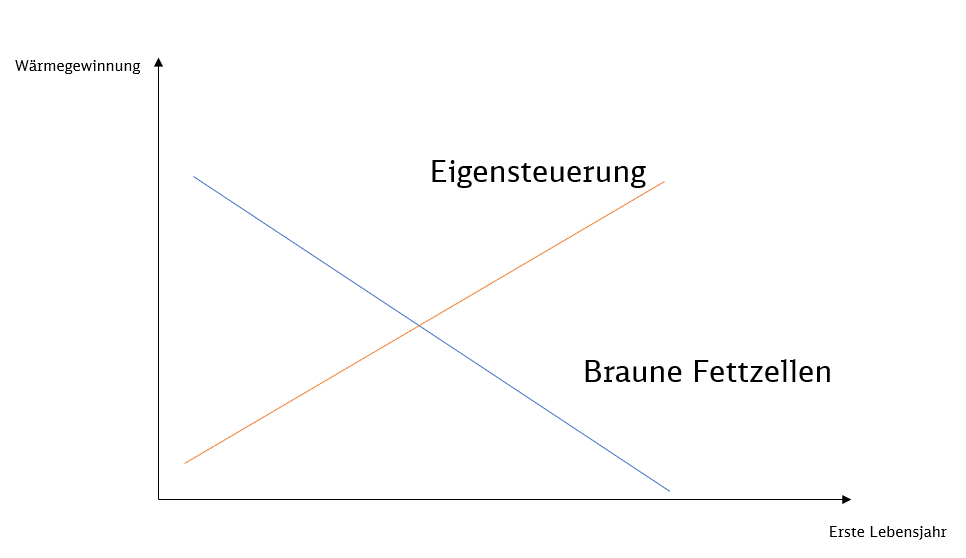
\includegraphics[scale = 0.3]{attachment/chapter_9/Scc001}
			\end{figure} 
		\end{itemize} \footnote{Empfehlung: Generell fühlen sich Säuglinge gut angezogen bei einer Raumtemperatur von etwa 24 bis 25 Grad Celsius am wohlsten. Herrschen aber in den Räumen der Wohnung „normale“ Temperaturen, das heißt zwischen 20 und 23 Grad Celsius im Wohnzimmer und 17 bis 20 Grad im Schlafzimmer, sind ein Body oder ein Shirt aus Baumwolle genau das Richtige zum Unterziehen für das Baby. Darüber eignet sich dann ein recht enganliegender leichter Pullover, beziehungsweise ein nicht allzu dickes Sweatshirt optimal.}
		\item Immunsystem
		\begin{itemize}
			\item Das Immunsystem wird bis das Stillen abgeschlossen ist, von der Muttermilch unterstützt. Antikörper werden über die Milch übertragen.
			\item Gleichzeitig trägt der enge Bund dazu bei, dass die Mutter den gleichen Erregern ausgesetzt ist.
		\end{itemize}
		\item Plötzlicher Kindstod
		\begin{itemize}
			\item Genaue physische Ursachen sind für dieses Phanomän sind nicht ableitbar.
			\item Empfehlungen wie: \textit{Säuglinge} im ersten Lebensjahr sollen immer auf dem Rücken einschlafen, und es soll kontrolliert werden, dass dies auch durch die Nacht hin passiert. Es ist dabei möglich, dass auf dem Bauch zuerst eingeschlafen wird und später der Säugling umgedreht wird. 
			\item Tagsüber ist für die Ausbildung der Rückenmuskulatur entscheidend, dass der Säugling auf dem Bauch liegt. 
		\end{itemize}
	\end{itemize}
	\item[6 Wochen]
	\begin{itemize}
		\item Iterationen mit unvertrauten Umgebungen sind eine hohe Lernherausforderung. Beispiel: Ein Besuch im Supermarkt zählt zu solchen Lerneindrücken.
		\item Die Hörqualität wird mit weiterem Alter nur noch abnehmen, und ist somit nie wieder so gut, wie als Neugeborenes.
		\item Retina und die Muskulatur zum Einstellen der Linse ist noch nicht entwickelt und trainiert. Diese führt dazu, dass schwarz-weiß und unscharf gesehen wird.
		\item Nach ca. 2 Monaten können Farben auseinander gehalten werden.
		\item Nach ca. 4 Monaten können Gesichter auseinander gehalten werden.
		\item In den ersten drei Monaten herrscht eine Wachstumsrate von 25 $\%$ je Monat
		\item Ab 6 Monaten kann sich ein Säugling meist drehen. Dies erhöht das Risiko für einen plötzlichen Kindstod.
	\end{itemize}
	\item[8 Monate]
	\begin{itemize}
		\item Alle Sinne sind vollständig ausgebildet.
		\item Mit dem Tastsinn werden weitere Lernprozesse angestoßen.
		\item Weil die Dichte im Mund an Sinneszellen sehr hoch ist, wird dieser genutzt, um eine höhere Lernqualität zu erhalten. Der Mund besitzt spezielle Enzyme, welche Bakterien angreifen.
		\item Mit dem 9 Lebensmonat startet die Aushärtung der Kopfform und Knochenbildung. Dies führt dazu, dass Asymetrien sich ab diesen Zeitpunkt verfestigen. Bis zum Ende des ersten Jahres ist dieser Prozess abgeschlossen.
	\end{itemize}
	\item[1 Jahr]
	\begin{itemize}
		\item Durch die Möglichkeit des Krabbels startet die Entwicklung von einem Baby zu einem Kleinkind.
		\item Fähigkeit des Sprechens wird entwickelt
	\end{itemize}
	\item[11 Jahre]
	\begin{itemize}
		\item Hormonbildung startet.
		\item Die sexuelle Entwicklung startet.
	\end{itemize}
\end{enumerate}
\footnote{
	Quelle 1: \href{https://www.ipzf.de/gehirnentwicklung.html}{Link},
	Quelle 2: \href{https://www.youtube.com/watch?v=ZNYv_ory8rc}{Living Body Documentation},
	Quelle 3: %\href{https://kinderzeit-bremen.de/familienzeit/schwanger-und-baby/waermehaushalt-bei-neugeborenen-tipps-risiken/#:~:text=Gerade\%20in\%20den\%20ersten\%20neun,kommt\%20es\%20rasch\%20zu\%20Temperaturverlust.}{Wärmehaushalt bei Neugeborenen}
	%Quelle 4: \href{https://www.varilag.de/ratgeber/baby-kopfform/#:~:text=Die\%20Sch\%C3\%A4delbasis\%20entwickelt\%20sich\%20aus,die\%20den\%20Sch\%C3\%A4del\%20flexibel\%20halten.}{Die Kopfform von Babys}
}

\subsection{Bedingungslose Liebe in der EKB} Wie kann dies unter Berücksichtigung der drei \gls{p_Obj} verstanden werden?\\

% Die Chance, immer eine Rückfall-Ebene zu haben
% Das bedeutet aber nicht, dass man auch gemocht wird und Leute gern mit einem Zeitverbringen wollen (Freundschaft) oder die Leistungen von einem wertschätzen (Drive))

Dieser Bestandteil der \gls{p_EKB} kann sich positive auf \NFMOTwo auswirken, muss es aber nicht.\\
Es ist ebenso möglich, dass sich keine positive Beziehung mit natürlicher Sympathie einstellt, in welche die \gls{p_FM} sich gegenseitig Kraft geben. Ist dies der Fall, soll für \gls{p_NFM} sich jedoch gewiss fühlen, dass wir immer der eine bedingungslose Liebe zwischen den \gls{p_FM} herrscht.\\

Dabei ist es für \NFMOOne wichtig zu verstehen, dass dies nicht bedeutet, dass trotz keiner Anstrengung, alle einen sympathisch finden, gern mit einen Zeit verbracht wollen oder Respekt gegenüber den Leistungen vorherrscht. Es bedeutet, dass immer Hilfe und Unterstützung von den \gls{p_FM} einen entgegen gebracht wird und immer eine besonderen Beziehung zwischen den Eltern und \gls{p_NFM} vorherrscht.\\

Es besteht das Risiko, dass bei einer permanenten Rückfall-Ebenen, sich kein eigener Antrieb entwickelt. Wie im vorherigen Absatz beschrieben, wird damit nicht der Respekt für die eigenen Leistungen abgedeckt oder sich automatische eine \gls{p_FB} einstellen, in welcher die \gls{p_FM} gern mit einem Zeit verbringen wollen. Ist \gls{p_NFM} dies wichtig, besteht für es keine Garantie, dass dies Teil in der \gls{p_EKB} oder in der \gls{p_FB} wird.

\subsection{\gls{p_FB}} Neben der \gls{p_EKB} gibt es jedoch auch die \gls{p_FB}, der \gls{p_FM} untereinander. Beide Beziehungen können zwischen den \gls{p_FM} zur gleichen Zeit existieren.

\subsection{Wettbewerb mit uns (NFM)}
Unsere Strategie ist kein Geheimnis. Ganz im Gegenteil, es ist kein Grund bekannt, welche uns in eine schlechtere Lage versetzt, diese Strategie zu teilen. Hierbei ist zu vermerken, dies ist nicht immer der Fall: Besonders im Wettbewerb mit anderen Parteien kann es von Nachteil sein, wenn andere Parteien die Vorhaben kennen, besonders, wenn all das gleiche Ziel haben.\\

In unserem Fall stehe wir nicht mit anderen im Wettbewerb, sondern mit uns im Zeitverlauf. Unser Ziel, siehe \ref{part:NFM_sec:Objective}, ist nicht zeitgebunden jedoch außerhalb unsere Kontrolle. Dennoch können wir $"$verlieren$"$. Dies würde zu uns selbst passieren. Wir erreichen nicht den gewünschten Zustand in unserem Leben, welcher uns die größte Freude und Erfüllung bereitet - und warum sollte man danach nicht streben. Es gibt jedoch genügend Irrwege, Hindernisse und Risiken, welche uns daran hindern, unseren Wunsch-Zustand zu erreichen. Diese sollen in einer strategischen Betrachtung erkannt und adressiert werden. Welches nicht bedeutet, dass diese immer gelöst oder umgangen werden können. Unser Anstrengungen zielen darauf ab, kontinuierlich nach den besten subobtimalsten Zustand zustreben.\\

\subsection{Ungleichgewicht}

Es besteht die Annahme, dass wenn keine Gegenmaßnahmen ergriffen oder ein Bewusstsein für diese Ungleichgewicht geschaffen wird, es außer Kontrolle gerät oder ewig verhart, welches \NFMOTwo gefährdet. 
Das Risiko besteht, wird diese Ungleichgewicht nicht rechtzeitig reduziert oder nicht weise eingesetzt wird, um \NFMOOne zu erreichen, dass \NFMOTwo nicht erreicht wird.\\

\subsection{TSU}

Temporär Spielumgebung schaffen

Quelle: ICE Fahrt nach Weihnachten

NFM kann sich sicher selbst beschäftigen, jedoch benötigt es unsere Unterstützung Temporäre Spielumgebungen zu schaffen. Im weitern Verlauf (Vielleicht Zeitabschnitte benennen) kann und wird von uns dazu hinentwickelt, dass es sich eigene TSUs bauen kann. Die Ressourcen Bindung wird sein, diese dem NFM zu Verfügung zu stellen und diese über den gegeben Zeitraum aufrecht zuhalten. Je nach Konzeption, kann ein TSU physischer oder auch mentaler Natur sein. Z.B.: Eine Spielecke, im Raum tanzen, Laut singen. 

Hierbei ist unsere Aufgabe die Interationsfluss mit der Gesellschaft zu managen, um eine TSU für das NFM und die angrenzende Gesellschaft aufrechtzuerhalten und jeweilige Präferenzen gegegenüber NFM und der Gesellschaft zu optimieren.

Z.B.: Freie Entwicklung zu singen, um NFM die Möglichkeit im Zug zu geben, sich auszuprobieren und den Geräusch Pegel so anzupassen, dass andere angrenzen Personen, sich so wohl damit fühlen, sodass diese nicht versuchen den TSU aufzulösen.

\subsection{Mantra}
Die Mantras sind nur Phrasen, welche eine Verlinkung im Kopf herstellen, zu einem größeren Thema oder eine emotionale Hürde im Moment überwinden.


\paragraph{Beste für Dich}
Im Herzen von jedem in der Familie sollte, das der Wunsch vorhanden sein, dass \textit{Beste} für die anderen \gls{p_FM} zu wollen.\\

Dies ist schon in einer zweiter Dynamik schwer, in der mind. dreier Dynamik mit dem \NFMOOne ist dies eine andere Herausforderung. Sich daran zu erinnern, ist jedoch das \textit{Mantra}, an welches sich permanent erinnert werden muss.


\paragraph{Sammlung} 
Nicht alle Mantras sind ausformuliert, wie das obrige. Diese werden hier als Liste aufgeführt. Das Ziel davon ist, diese im Alltag auszuprobieren oder weiter zu vertesten. 

\begin{itemize}
	\item Du bist eine Bereicherung
	\item Eigenständig $\&$ Kompetent
	\item With all that is given to you, you make it your own. (Marvel, Shing Chan)
	\item Gemeinsame Zeit gibt uns Kraft (Z)
\end{itemize}

\subsection{Entwicklungstufen}

\begin{itemize}
	\item[Neugeborenes] $[0, 28 \text{Lebenstag}]$
	\item[Saugling] $[0,365 \text{Lebenstag}]$
	\item[Kleinkind] $[1 \text{Lebensjahr}, 3 \text{Lebensjahr}]$
	\item[Kind] $[4 \text{Lebensjahr}, 12 \text{Lebensjahr}]$
	\item[Jugentlicher] $[13 \text{Lebensjahr}, 17 \text{Lebensjahr}]$
	\item[Erwachsener] $[18 \text{Lebensjahr}, \dots )$
\end{itemize}


\subsection{Lernthemen}
\begin{description}
	\item[Work-Concept / General] Sometimes it is a choice to have truely feel love  for someone. This can even work at work. This give you the ability to overlook topics that are not working well, if there are not so important for you goals. This doesn't mean, you trust blindly. The oposide, you then specially have a higher standard to evaluate there action (Hugo Mercier) 
	\item Ist das das beste was du tuen konntest: die letzten 5 % sind die Prozent, die zählen
\end{description}